\documentclass[pdf]{beamer}
\mode<presentation>{} 

\usepackage{hyperref}
\usepackage{pgf}
\usepackage{tikz}
\usetikzlibrary{trees}
\usetikzlibrary{arrows,automata}
\usetikzlibrary{automata,positioning}
\usetikzlibrary{shapes}
\usepackage{tikz-qtree,tikz-qtree-compat}
\usepackage{mathtools,enumerate,amssymb}
\usepackage[utf8]{inputenc}
\usepackage[T1]{fontenc}
\usepackage{graphicx}
\usepackage{multirow}
\usepackage[export]{adjustbox}
\usepackage{wrapfig}
\usepackage{multicol}
\definecolor{Blue}{RGB}{0,0,100}
\definecolor{background}{RGB}{255,255,255}

\title{Evaluating interfaces with the users - Qualitative Methods}
\subtitle{Human Computer Interaction}
\AtBeginSection[]{}



\setbeamertemplate{sidebar right}{}
\setbeamertemplate{footline}{%
\hfill\usebeamertemplate***{navigation symbols}
\hspace{1cm}\insertframenumber{}/\inserttotalframenumber}

\graphicspath{{./img/}}



\begin{document}

{\setbeamercolor{background canvas}{bg=background}
\begin{frame}
\vspace{10mm}
\huge{\raggedleft{\color{black}{\textbf{Evaluating interfaces with the users - Qualitative Methods}}}}

\large{\raggedleft{\color{black} Human Computer Interaction}}

\begin{flushright}
\end{flushright}

\fontsize{7pt}{1pt}\selectfont{
Based on slide deck 

\textbf{Part 3: Designing with the user. Evaluating interfaces with the users - Qualitative Methods}

Human Computer Interaction I: Principles and Design

by

\textbf{Saul Greenberg}
\newline
Professor
\newline
\textbf{University of Calgary, Canada}

\textit{The new slides are marked with a *}
}

\fontsize{5pt}{1pt}\selectfont{ \textcolor{lightgray}
{Slide deck by Saul Greenberg. Permission is granted to use this for non-commercial purposes as long as general credit to Saul Greenberg is clearly maintained.
Warning: some material in this deck is used from other sources without permission. Credit to the original source is given if it is known.}}

\end{frame}}

% Inaintea codului fiecarui slide se vor scrie urmatoarele informatii:
% Nume si prenume student
% Numarul slide-ului corespunzator din prezentarea prof. Saul Greenberg
% Numele imaginilor inserate trebuie sa fie numar_slide_nume_imagine.extensie_imagine


% Suciu Ioan
% slide 1
{\setbeamercolor{background canvas}{bg=background}
\setbeamercolor{normal text}{fg=Blue}
\usebeamercolor[fg]{normal text}
\begin{frame}
\bigskip
\bigskip
\bigskip
      \textbf{\LARGE Evaluating interfaces with the users \LARGE}
\bigskip
\bigskip
\bigskip

Why evaluation is crucial 

Quickly debug prototypes by observing people use them

Methods that reveal what a person is thinking about 

Ethics
    \begin{figure}[b]
    	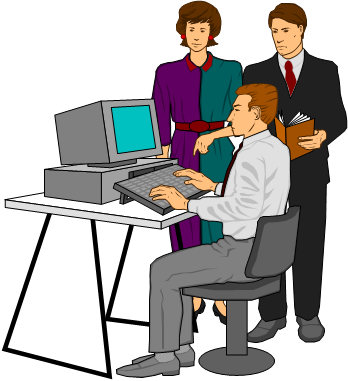
\includegraphics[scale = 0.4, right]{1_img.png}
    \end{figure}
\end{frame}}



%% Suciu Ioan
%% slide 3
%{\setbeamercolor{background canvas}{bg=background}
%\setbeamercolor{normal text}{fg=Blue}
%\usebeamercolor[fg]{normal text}
%\begin{frame}
%    \textcolor{Blue}{\textbf{\Large{Why bother?}}}
%    \textcolor{red}{\rule{10cm}{1mm}}
%    Tied to the usability engineering lifecycle\par
%    \bigskip
%	\bigskip
%	\bigskip
%    Pre-design\par
%    \begin{itemize}
%    \item[\textcolor{black}{--}] investing in new expensive system requires proof of viability 
%    \end{itemize}
%    	\bigskip
%   Initial design stages\par
%    \begin{itemize}
%    \item[\textcolor{black}{--}] develop and evaluate initial design ideas with the user
%    \end{itemize}
%    \begin{figure}[b]
%    	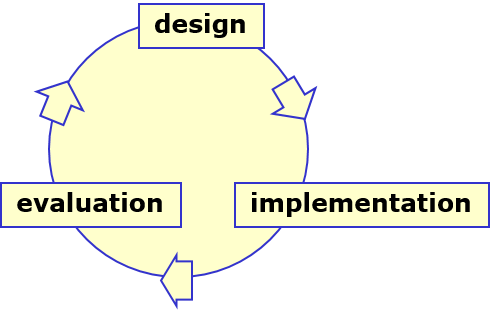
\includegraphics[scale = 0.4, right]{3_4_img.png}
%    \end{figure}
%\end{frame}}


% Suciu Ioan
% slide 4
{\setbeamercolor{background canvas}{bg=background}
\setbeamercolor{normal text}{fg=Blue}
\usebeamercolor[fg]{normal text}
\begin{frame}
    \textcolor{Blue}{\textbf{\Large{Why bother?}}}
    \textcolor{red}{\rule{10cm}{1mm}}
    
    \textbf{Iterative design}\par
    \begin{itemize}
    \item[\textcolor{black}{--}] does system behavior match the user’s task requirements?
    \item[\textcolor{black}{--}] are there specific problems with the design? 
    \item[\textcolor{black}{--}] what solutions work? 
    \end{itemize}
    	\bigskip
   \textbf{Acceptance testing}\par
    \begin{itemize}
    \item[\textcolor{black}{--}] verify that system meets expected user performance criteria
    \begin{itemize}
    	\item[\textcolor{black}{•}] 80\% of 1st time customers will take 1-3 minutes to  withdraw \$50 from the automatic teller
    \end{itemize}
    \end{itemize}
    \begin{figure}[b]
    	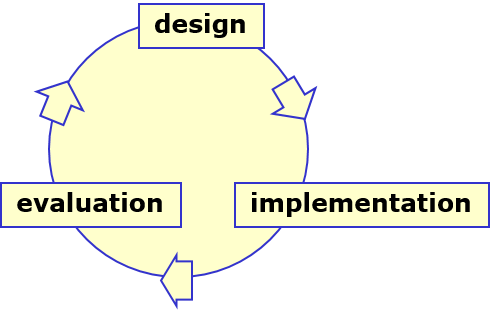
\includegraphics[scale = 0.4, right]{3_4_img.png}
    \end{figure}
\end{frame}}



{\setbeamercolor{background canvas}{bg=background}
\setbeamercolor{normal text}{fg=Blue}
\usebeamercolor[fg]{normal text}
\begin{frame}
    \textcolor{Blue}{\textbf{\Large{*Evaluation}}}
    \textcolor{red}{\rule{10cm}{1mm}}

\large{\textbf{Naturalistic approach}}
\newline
\newline
\large{\textbf{Experimental approach}}
\begin{itemize}
	\item
		\large{usability engineering}
			\begin{itemize}
				\item usability inspection methods
					\begin{itemize}
						\item qualitative methods
						\item quantitative methods
					\end{itemize}
				\item usability testing methods
					\begin{itemize}
						\item qualitative methods
						\item quantitative methods
					\end{itemize}
			\end{itemize}
	\end{itemize}
\end{frame}



% Suciu Ioan
% slide 5
{\setbeamercolor{background canvas}{bg=background}
\setbeamercolor{normal text}{fg=Blue}
\usebeamercolor[fg]{normal text}
\begin{frame}
    \textcolor{Blue}{\textbf{\Large{Naturalistic approach}}}
    \textcolor{red}{\rule{10cm}{1mm}}
    
    Observation occurs in realistic setting\par
    \begin{itemize}
    \item[\textcolor{black}{--}] real life
    \end{itemize}
    	\bigskip
   Problems\par
    \begin{itemize}
    \item[\textcolor{black}{--}] hard to arrange and do
    \item[\textcolor{black}{--}] time consuming
    \item[\textcolor{black}{--}] may not generalize
    \end{itemize}
    \begin{figure}[b]
    	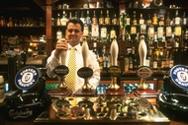
\includegraphics[scale = 0.4, right]{5_img.png}
    \end{figure}    
\end{frame}}



% Suciu Ioan
% slide 6
{\setbeamercolor{background canvas}{bg=background}
\setbeamercolor{normal text}{fg=Blue}
\usebeamercolor[fg]{normal text}
\begin{frame}
    \textcolor{Blue}{\textbf{\Large{Experimental approach}}}
    \textcolor{red}{\rule{10cm}{1mm}}
    
   Experimenter controls all environmental factors\par
    \begin{itemize}
    \item[\textcolor{black}{--}] study relations by manipulating \textit{independent} variables

    \item[\textcolor{black}{--}] observe effect on one or more \textit{dependent} variables

    \item[\textcolor{black}{--}] Nothing else changes
    \end{itemize}
    
    \bigskip
    \bigskip
    
    \textit{There is no difference in user performance (\textbf{time} and \textbf{error rate}) when selecting an item from a \textbf{pull down} or a \textbf{pull right} menu of 4 items}
    \begin{figure}[b]
    	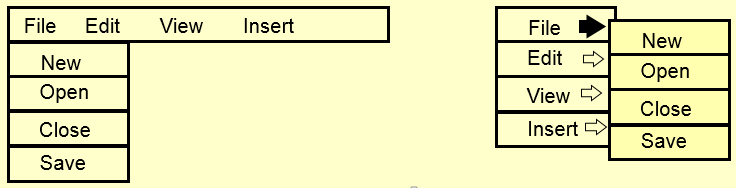
\includegraphics[scale = 0.4, center]{6_img.png}
    \end{figure}    
\end{frame}}



% Suciu Ioan
% slide 7
{\setbeamercolor{background canvas}{bg=background}
\setbeamercolor{normal text}{fg=Blue}
\usebeamercolor[fg]{normal text}
\begin{frame}
    \textcolor{Blue}{\textbf{\Large{Validity}}}
    \textcolor{red}{\rule{10cm}{1mm}}
    
   \textit{External validity}\par
    \begin{itemize}
    \item[\textcolor{black}{--}] confidence that results applies to real situations
    \item[\textcolor{black}{--}] usually good in natural settings
    \end{itemize}
    
    \bigskip

       \textit{Internal validity}\par
    \begin{itemize}
    \item[\textcolor{black}{--}] confidence in our explanation of experimental results
    \item[\textcolor{black}{--}] usually good in experimental settings
    \end{itemize}
    
    \bigskip
    \bigskip
    
      Trade-off: Natural \textit{vs} Experimental\par
    \begin{itemize}
    \item[\textcolor{black}{--}] precision and direct control over experimental design 
    
    \textit{versus}
    
    \item[\textcolor{black}{--}] desire for maximum generalizability in real life situations
    \end{itemize}
    
    \bigskip
    \bigskip
\end{frame}}



{\setbeamercolor{background canvas}{bg=background}
\setbeamercolor{normal text}{fg=Blue}
\usebeamercolor[fg]{normal text}
\begin{frame}
    \textcolor{Blue}{\textbf{\Large{*Usability engineering approach}}}
    \textcolor{red}{\rule{10cm}{1mm}}

	\begin{itemize}
	\item 
		\textbf{usability engineering} - iterative process to improve usability of a system
	
	\item
		\textbf{usability} - the extent to which a product can be used by specified users to achieve specified goals with \textit{effectiveness}, \textit{efficiency} and \textit{satisfaction} in a specified context of use [ISO 1998]
		
		\begin{itemize}
		\item
		\textbf{effectiveness} - accuracy and completeness in achieving specified goals
		\item
		\textbf{efficiency} -  resources expended in relation to the accuracy and completeness in achieving goals
		\item
		\textbf{satisfaction} - freedom from discomfort, and positive attitudes towards the use of the product
		\end{itemize}
	\end{itemize}
\end{frame}}



{\setbeamercolor{background canvas}{bg=background}
\setbeamercolor{normal text}{fg=Blue}
\usebeamercolor[fg]{normal text}
\begin{frame}
    \textcolor{Blue}{\textbf{\Large{*Usability engineering approach}}}
    \textcolor{red}{\rule{10cm}{1mm}}

\large {\textbf{Types of evaluation} (according to its purpose)}
\newline

	\begin{itemize}
	\item 
	\textbf{exploratory} - how is it (or will it be) used?
	\begin{itemize}
		\item explores current usage and the potential design space for new designs
		\newline
	\end{itemize}
	\item
	\textbf{predictive} - estimating how good it will be
	\begin{itemize}
		\item estimates the overall quality of an interface (once a design has been made)
		\newline
	\end{itemize}
	\item
	\textbf{formative} - how can it be made better?
	\begin{itemize}
		\item informs the design process and helps improve an interface 
during design
	\newline
	\end{itemize}
	\item
	\textbf{summative} - how good is it?
	\begin{itemize}
		\item assesses the overall quality of an interface
	\end{itemize}
	\end{itemize}
\end{frame}}



% Taran Alexandru
% slide 13
{\setbeamercolor{background canvas}{bg=background}
\setbeamercolor{normal text}{fg=Blue}
\usebeamercolor[fg]{normal text}
\begin{frame}
	\begin{tikzpicture}[remember picture,overlay,shift={(current page.south east)}]
      \node[anchor=south east,xshift=-0.5cm,yshift=0.5cm]{
\includegraphics[width=3cm, height=3cm]{13_img.png}};
    \end{tikzpicture}
    \textcolor{Blue}{\textbf{\Large{Usability inspection methods}}}
    \textcolor{red}{\rule{10cm}{1mm}}
    
    \textbf{Designer} tries the system (or prototype)\par
    \begin{itemize}
    \item[\textcolor{black}{--}] does the system "feel right"?
    \item[\textcolor{black}{--}] benefits
    	\begin{itemize}
    	\item[\textcolor{black}{•}] can catch some major problems in early versions
    	\end{itemize}
    \item[\textcolor{black}{--}] problems
    \begin{itemize}
    	\item[\textcolor{black}{•}] not reliable as completely subjective
        \item[\textcolor{black}{•}] not valid as introspector is a non-typical user
        \item[\textcolor{black}{•}] intuitions and introspection are often wrong
    \end{itemize}
    \end{itemize}
    \textbf{Usability inspection methods:}\par
    \begin{itemize}
    	\item[\textcolor{black}{--}] task centered walkthroughs
    	\item[\textcolor{black}{--}] heuristic evaluation
    \end{itemize}
\end{frame}}



% Taran Alexandru
% slide 8
{\setbeamercolor{background canvas}{bg=background}
\setbeamercolor{normal text}{fg=Blue}
\usebeamercolor[fg]{normal text}
\begin{frame}
    \textcolor{Blue}{\textbf{\Large{Usability testing methods}}}
    \textcolor{red}{\rule{10cm}{1mm}}
    Observe people using systems in \textbf{simulated} settings\par
    \begin{itemize}
    \item[\textcolor{black}{--}] people brought in to artificial setting that simulates aspects of real world setting
    \item[\textcolor{black}{--}] people given specific tasks to do
    \item[\textcolor{black}{--}] observations / measures made as people do their tasks
    \item[\textcolor{black}{--}] look for problem areas / successes
    \item[\textcolor{black}{--}] good for uncovering 'big effects'
    \end{itemize}
    \begin{figure}[b]
    	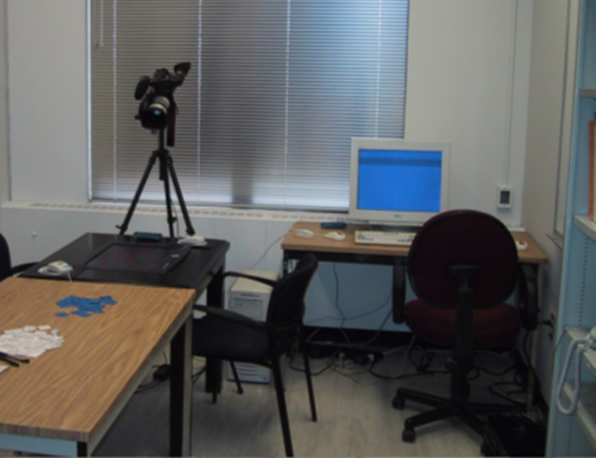
\includegraphics[scale = 0.4, right]{8_9_img.png}
    \end{figure}
\end{frame}}



% Taran Alexandru
% slide 9
{\setbeamercolor{background canvas}{bg=background}
\setbeamercolor{normal text}{fg=Blue}
\usebeamercolor[fg]{normal text}
\begin{frame}
	\begin{tikzpicture}[remember picture,overlay,shift={(current page.south east)}]
      \node[anchor=south east,xshift=-0.5cm,yshift=0.3cm]{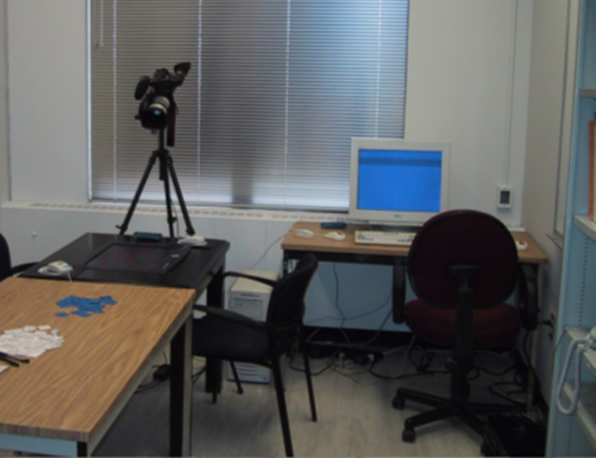
\includegraphics[width=4cm, height=3cm]{8_9_img.png}};
    \end{tikzpicture}
    \textcolor{Blue}{\textbf{\Large{Usability testing methods}}}
    \textcolor{red}{\rule{10cm}{1mm}}\par
    Is the test result relevant to the usability of real products in real use outside of lab?\par
    \textbf{Problems}\par
    \begin{itemize}
    \item[\textcolor{black}{--}] non-typical users tested
    \item[\textcolor{black}{--}] non-typical tasks
    \item[\textcolor{black}{--}] different physical environment
    \item[\textcolor{black}{--}] different social context
    	\begin{itemize}
    	\item[\textcolor{black}{•}] motivation towards experimenter vs motivation towards boss
    	\end{itemize}
    \end{itemize}
    \textbf{Partial solution}\par
    \begin{itemize}
    \item[\textcolor{black}{--}] use real users
    \item[\textcolor{black}{--}] task-centered system design tasks
    \item[\textcolor{black}{--}] environment similar to real situation
    \end{itemize}
\end{frame}}



% Taran Alexandru
% slide 10
{\setbeamercolor{background canvas}{bg=background}
\setbeamercolor{normal text}{fg=Blue}
\usebeamercolor[fg]{normal text}
\begin{frame}
	\begin{tikzpicture}[remember picture,overlay,shift={(current page.south east)}]
      \node[anchor=south east,xshift=0cm,yshift=0cm]{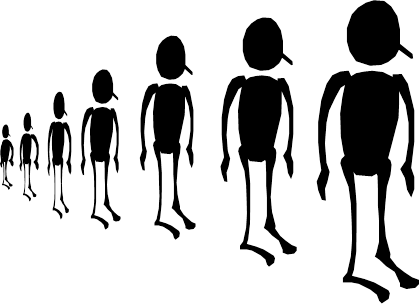
\includegraphics[width=3.5cm, height=2.5cm]{10_img.png}};
    \end{tikzpicture}
    \textcolor{Blue}{\textbf{\Large{Usability testing methods}}}
    \textcolor{red}{\rule{10cm}{1mm}}
    How many users should you observe?\par
    \begin{itemize}
    \item[\textcolor{black}{--}] observing many users is expensive
    \item[\textcolor{black}{--}] \textit{but} individual differences matter
    	\begin{itemize}
    	\item[\textcolor{black}{•}] best user 10x faster than slowest
        \item[\textcolor{black}{•}] best 25\% of users approx. 2x faster than slowest 25\%
    	\end{itemize}
    \end{itemize}
    Partial Solution\par
    \begin{itemize}
    \item[\textcolor{black}{--}] reasonable number of users tested
    \item[\textcolor{black}{--}] reasonable range of users
    \item[\textcolor{black}{--}] big problems usually detected with handful of users
    \item[\textcolor{black}{--}] small problems / fine measures need many users
    \end{itemize}
\end{frame}}



% Taran Alexandru
% slide 11
{\setbeamercolor{background canvas}{bg=background}
\setbeamercolor{normal text}{fg=Blue}
\usebeamercolor[fg]{normal text}
\begin{frame}
    \textcolor{Blue}{\textbf{\Large{Usability testing methods}}}
    \textcolor{red}{\rule{10cm}{1mm}}\par
    Low cost methods to gather usability problems\par
    \begin{itemize}
    	\item[\textcolor{black}{--}] approximate: capture most large and many minor problems
    \end{itemize}
    How?\par
    \begin{itemize}
    \item[\textcolor{black}{--}] \textbf{qualitative}:
    	\begin{itemize}
    	\item[\textcolor{black}{•}] observe user interactions 
        \item[\textcolor{black}{•}] gather user explanations and opinions 
        \item[\textcolor{black}{•}] produces a description, usually in non-numeric terms
        \item[\textcolor{black}{•}] anecdotes, transcripts, problem areas, critical incidents…
        \end{itemize}
    \item[\textcolor{black}{--}] \textbf{quantitative}
    	\begin{itemize}
    	\item[\textcolor{black}{•}] count, log, measure something of interest in user actions
        \item[\textcolor{black}{•}] speed, error rate, counts of activities
        \end{itemize}
    \end{itemize}
\end{frame}}



% Taran Alexandru
% slide 12
{\setbeamercolor{background canvas}{bg=background}
\setbeamercolor{normal text}{fg=Blue}
\usebeamercolor[fg]{normal text}
\begin{frame}
    \textcolor{Blue}{\textbf{\Large{Qualitative usability testing methods}}}
    \textcolor{red}{\rule{10cm}{1mm}}
    Methods\par
    \begin{itemize}
        \item[\textcolor{black}{--}] extracting the conceptual model
        \item[\textcolor{black}{--}] direct observation
        \begin{itemize}
    		\item[\textcolor{black}{•}] think-aloud
        	\item[\textcolor{black}{•}] constructive interaction/co-discovery
        \end{itemize}
        \item[\textcolor{black}{--}] query techniques (interviews and questionnaires)
        \item[\textcolor{black}{--}] continuous evaluation (user feedback and field studies)
    \end{itemize}
\end{frame}}



% Taran Alexandru
% slide 14
{\setbeamercolor{background canvas}{bg=background}
\setbeamercolor{normal text}{fg=Blue}
\usebeamercolor[fg]{normal text}
\begin{frame}
    \textcolor{Blue}{\textbf{\Large{Conceptual model extraction}}}
    \textcolor{red}{\rule{10cm}{1mm}}
    How?\par
    \begin{itemize}
    \item[\textcolor{black}{--}] show the user static images of
    	\begin{itemize}
    	\item[\textcolor{black}{•}] the prototype \textit{or} screens during use
    	\end{itemize}
    \item[\textcolor{black}{--}] ask the user explain 
    	\begin{itemize}
    	\item[\textcolor{black}{•}] the function of each screen element
        \item[\textcolor{black}{•}] how they would perform a particular task
    	\end{itemize}
    \end{itemize}
    What?\par
    \begin{itemize}
    \item[\textcolor{black}{--}] \textbf{Initial conceptual model}
    	\begin{itemize}
    	\item[\textcolor{black}{•}] how person perceives a screen the very first time it is viewed
    	\end{itemize}
    \item[\textcolor{black}{--}] \textbf{Formative conceptual model} 
    	\begin{itemize}
    	\item[\textcolor{black}{•}] How person perceives a screen after its been used for a while
    	\end{itemize}
    \end{itemize}
    Value?\par
    \begin{itemize}
    \item[\textcolor{black}{--}] good for eliciting people’s understanding before \& after use
    \item[\textcolor{black}{--}] poor for examining system exploration and learning
    \end{itemize}
\end{frame}}

% Taran Alexandru
% slide 15
{\setbeamercolor{background canvas}{bg=background}
\setbeamercolor{normal text}{fg=Blue}
\usebeamercolor[fg]{normal text}
\begin{frame}
	\textcolor{Blue}{\textbf{\Large{Direct observations}}}
    \textcolor{red}{\rule{10cm}{1mm}}
    Evaluator observes users interacting with system\par
    \begin{itemize}
    \item[\textcolor{black}{--}] in lab:
    	\begin{itemize}
    	\item[\textcolor{black}{•}] user asked to complete a set of pre-determined tasks
    	\end{itemize}
    \item[\textcolor{black}{--}] in field: 
    	\begin{itemize}
    	\item[\textcolor{black}{•}] user goes through normal duties
    	\end{itemize}
    \end{itemize}
    Value\par
    \begin{itemize}
    \item[\textcolor{black}{--}] excellent at identifying gross design/interface problems
    \item[\textcolor{black}{--}] validity depends on how controlled/contrived the situation is
    \end{itemize}
\end{frame}}

% Tesila Dan-Mihai
% slide 16
{\setbeamercolor{background canvas}{bg=background}
\setbeamercolor{normal text}{fg=Blue}
\usebeamercolor[fg]{normal text}
\begin{frame}
	\vspace{8mm}
	\textcolor{Blue}{\textbf{\Large{Simple observation method}}}
    \textcolor{red}{\rule{10cm}{1mm}}
    User is given the task \par
    Evaluator just watches the user \par
    \bigskip
    Problem
    \begin{itemize}
    \item[\textcolor{Blue}{--}] does not give insight into the user's decision process and attitude
    \end{itemize}
    \begin{figure}[b]
    	
\includegraphics[scale = 0.4, right]{16_imagine.png}
    \end{figure}
\end{frame}}

% Tesila Dan-Mihai
% slide 17
{\setbeamercolor{background canvas}{bg=background}
\setbeamercolor{normal text}{fg=Blue}
\usebeamercolor[fg]{normal text}
\begin{frame}
	\vspace{8mm}
	\textcolor{Blue}{\textbf{\large{Think aloud method}}}
    \textcolor{red}{\rule{10cm}{1mm}}
    Users speak their thoughts while doing the task \par
    \begin{itemize}
      \item[\textcolor{Blue}{--}] what they are trying to do
      \item[\textcolor{Blue}{--}] why they took an action
      \item[\textcolor{Blue}{--}] how they interpret what the system did
      \item[\textcolor{Blue}{--}] gives insight into what the user is thinking
      \item[\textcolor{Blue}{--}] most widely used evaluation method in industry
      \begin{itemize}
        \item[\textcolor{Blue}{\textbullet}] may alter the way users do the task
        \item[\textcolor{Blue}{\textbullet}] unnatural (awkward and uncomfortable)
        \item[\textcolor{Blue}{\textbullet}] hard to talk if they are concentrating
      \end{itemize}
    \end{itemize}
    \vspace{-0.3cm}
    \begin{figure}[b]
    	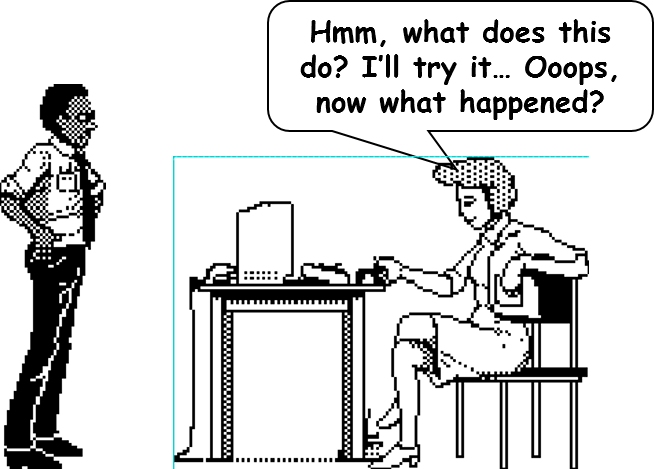
\includegraphics[scale = 0.4, right]{17_Imagine.png}
    \end{figure}
\end{frame}}



% Tesila Dan-Mihai
% slide 18
{\setbeamercolor{background canvas}{bg=background}
\setbeamercolor{normal text}{fg=Blue}
\usebeamercolor[fg]{normal text}
\begin{frame}
	\vspace{8mm}
	\textcolor{Blue}{\textbf{\large{Constructive interaction/Co-discovery method}}}
    \textcolor{red}{\rule{10cm}{1mm}}
    
    Two people work together on a task \par
    \begin{itemize}
      \item[\textcolor{Blue}{--}] monitor their normal conversations
      \item[\textcolor{Blue}{--}] removes awkwardness of think-aloud
    \end{itemize}
    \bigskip
    \begin{figure}[b]
    	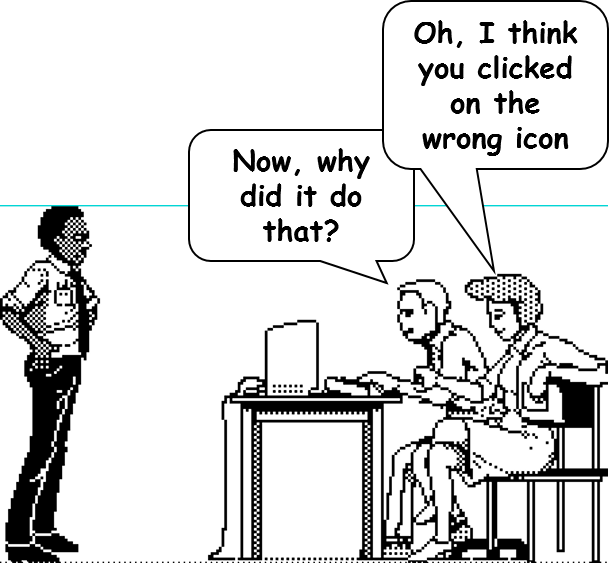
\includegraphics[scale = 0.4, right]{18_Imagine.png}
    \end{figure}
\end{frame}}



{\setbeamercolor{background canvas}{bg=background}
\setbeamercolor{normal text}{fg=Blue}
\usebeamercolor[fg]{normal text}
\begin{frame}
	\vspace{8mm}
	\textcolor{Blue}{\textbf{\large{Constructive interaction/Co-discovery method}}}
    \textcolor{red}{\rule{10cm}{1mm}}

    Co-discovery learning
    \begin{itemize}
      \item[\textcolor{Blue}{--}] use semi-knowledgeable "coach" and novice
      \item[\textcolor{Blue}{--}] only novice uses the interface
      \begin{itemize}
      	\item[{\textbullet}] novice asks questions
      	\item[{\textbullet}] coach responds
      \end{itemize}
      \item[\textcolor{Blue}{--}] gives insights into two user groups
    \end{itemize}
\end{frame}}



% Tesila Dan-Mihai
% slide 19
{\setbeamercolor{background canvas}{bg=background}
\setbeamercolor{normal text}{fg=Blue}
\usebeamercolor[fg]{normal text}
\begin{frame}
	\vspace{8mm}
	\textcolor{Blue}{\textbf{\large{Recording observations}}}
    \textcolor{red}{\rule{10cm}{1mm}}
    How do we record user actions for later analysis?
    \begin{wrapfigure}{b}{0.1\textwidth}
      \centering
      
\includegraphics[scale = 0.6, right]{19_toate.png}
    \end{wrapfigure}
    \begin{itemize}
      \item[\textcolor{Blue}{--}] otherwise risk forgetting, missing, or misinterpreting events
      \item[\textcolor{Blue}{--}] paper and pencil
      \begin{itemize}
        \item[\textcolor{Blue}{\textbullet}] primitive but cheap
        \item[\textcolor{Blue}{\textbullet}] observer records events, comments, and interpretations
        \item[\textcolor{Blue}{\textbullet}] hard to get detail (writing is slow)
        \item[\textcolor{Blue}{\textbullet}] 2\textsuperscript{nd} observer helps...
      \end{itemize}
      \item[\textcolor{Blue}{--}] audio recording
      \begin{itemize}
        \item[\textcolor{Blue}{\textbullet}] good for recording think aloud talk
        \item[\textcolor{Blue}{\textbullet}] hard to tie into on-screen user actions
      \end{itemize}
      \item[\textcolor{Blue}{--}] video recording
      \begin{itemize}
        \item[\textcolor{Blue}{\textbullet}] can see and hear what a user is doing
        \item[\textcolor{Blue}{\textbullet}] one camera for screen, rear view mirror useful
        \item[\textcolor{Blue}{\textbullet}] initially intrusive
      \end{itemize}
    \end{itemize}
\end{frame}}



% Tesila Dan-Mihai
% slide 20
{\setbeamercolor{background canvas}{bg=background}
\setbeamercolor{normal text}{fg=Blue}
\usebeamercolor[fg]{normal text}
\begin{frame}
	\vspace{8mm}
	\textcolor{Blue}{\textbf{\large{Coding sheet example...}}}
    \textcolor{red}{\rule{10cm}{1mm}}
    tracking a person's use of an editor
    \begin{center}
    \resizebox{\textwidth}{!}{
    \color{black}
    \begin{tabular} { c c c c|c c c|c c }
    & \multicolumn{3}{c}{General actions} & \multicolumn{3}{c}{Graph editing} & \multicolumn{2}{c}{Errors} \\
    Time & text & scrolling & image & new & delete & modify & correct & miss \\
    & editing & & editing & node & node & node & error & error\\
    09:00 & \textcolor{red}{\textbf{X}} & & & & & & & \\
    \hline
    09:02 & & & & \textcolor{red}{\textbf{X}} & & & & \\
    \hline
    09:05 & & & & & & & \textcolor{red}{\textbf{X}} & \\
    \hline
    09:10 & & & & & \textcolor{red}{\textbf{X}} & & & \\
    \hline
    09:13 & & & & & & & & 
    
    \end{tabular}
    }
    \end{center}
\end{frame}}



% Tesila Dan-Mihai
% slide 21
{\setbeamercolor{background canvas}{bg=background}
\setbeamercolor{normal text}{fg=Blue}
\usebeamercolor[fg]{normal text}
\begin{frame}
	\vspace{8mm}
	\textcolor{Blue}{\textbf{\large{Interviews}}}
    \textcolor{red}{\rule{10cm}{1mm}}
    Good for pursuing specific issues
    \begin{itemize}
      \item[\textcolor{Blue}{--}] vary questions to suit the context
      \item[\textcolor{Blue}{--}] probe mode deeply on interesting issues as they arise
      \item[\textcolor{Blue}{--}] good for exploratory studies via open-ended questioning
      \item[\textcolor{Blue}{--}] often leads to specific constructive suggestions
    \end{itemize}
    \bigskip
    Problems:
    \begin{itemize}
      \item[\textcolor{Blue}{--}] accounts are subjective
      \item[\textcolor{Blue}{--}] time consuming
      \item[\textcolor{Blue}{--}] evaluator can easily bias the interview
      \item[\textcolor{Blue}{--}] prone to rationalization of events/thoughts by user
      \begin{itemize}
      	\item[\textcolor{Blue}{\textbullet}] user's reconstruction may be wrong
      \end{itemize}
    \end{itemize}
    \vspace{-0.3cm}
    \begin{figure}[b]
    	
\includegraphics[scale = 0.4, right]{21_Imagine.png}
    \end{figure}
\end{frame}}



% Tesila Dan-Mihai
% slide 22
{\setbeamercolor{background canvas}{bg=background}
\setbeamercolor{normal text}{fg=Blue}
\usebeamercolor[fg]{normal text}
\begin{frame}
	\vspace{8mm}
	\textcolor{Blue}{\textbf{\large{How to interview}}}
    \textcolor{red}{\rule{10cm}{1mm}}
    Plan a set of central questions
    \begin{itemize}
      \item[\textcolor{Blue}{--}] a few good questions gets things started
      \begin{itemize}
      	\item[\textcolor{Blue}{\textbullet}] avoid leading questions
      \end{itemize}
      \item[\textcolor{Blue}{--}] focuses the interview
      \item[\textcolor{Blue}{--}] could be based on results of user observations
    \end{itemize}
    \bigskip
    Let user responses lead follow-up questions
    \begin{itemize}
      \item[\textcolor{Blue}{--}] follow interesting leads \textit{vs} bulldozing through question list
    \end{itemize}
    \begin{figure}[b]
    	
\includegraphics[scale = 0.4, right]{21_Imagine.png}
    \end{figure}
\end{frame}}



% Tesila Dan-Mihai
% slide 23
{\setbeamercolor{background canvas}{bg=background}
\setbeamercolor{normal text}{fg=Blue}
\usebeamercolor[fg]{normal text}
\begin{frame}
	\vspace{8mm}
	\textcolor{Blue}{\textbf{\large{Retrospective testing interviews}}}
    \textcolor{red}{\rule{10cm}{1mm}}
    Post-observation interview to
    \begin{itemize}
      \item[\textcolor{Blue}{--}] perform an observational test
      \item[\textcolor{Blue}{--}] create a video record of it
      \item[\textcolor{Blue}{--}] have users view the video and comment on what they did
      \begin{itemize}
        \item[\textcolor{Blue}{\textbullet}] clarify events that occured during system use
        \item[\textcolor{Blue}{\textbullet}] excellent for grounding a post-test interview
        \item[\textcolor{Blue}{\textbullet}] avoids erroneous reconstruction
        \item[\textcolor{Blue}{\textbullet}] users often offer concrete suggestions
      \end{itemize}
    \end{itemize}
    \vspace{-1.5cm}
    \begin{figure}[b]
    	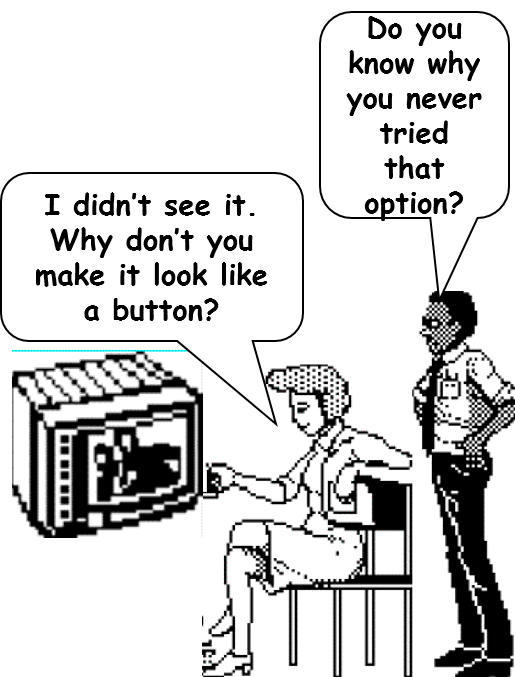
\includegraphics[scale = 0.4, right]{23_Imagine.png}
    \end{figure}
\end{frame}}


%/////////////////////////////////////////////////////////////
% Toader Marina Adina
% slide 24
{\setbeamercolor{background canvas}{bg=background}
\setbeamercolor{normal text}{fg=Blue}
\usebeamercolor[fg]{normal text}
\begin{frame}
	\vspace{8mm}
	\textcolor{Blue}{\textbf{\large{Critical incidence interviews}}}
    \textcolor{red}{\rule{10cm}{1mm}}
    
    People talk about incidents that stood out
    \begin{itemize}
      \item[\textcolor{black}{--}] usually discuss extremely annoying problems with fervor
      \item[\textcolor{black}{--}] not representative, but important to them
      \item[\textcolor{black}{--}] often raises issues not seen in lab tests
    \end{itemize}
    \begin{figure}[b]
    	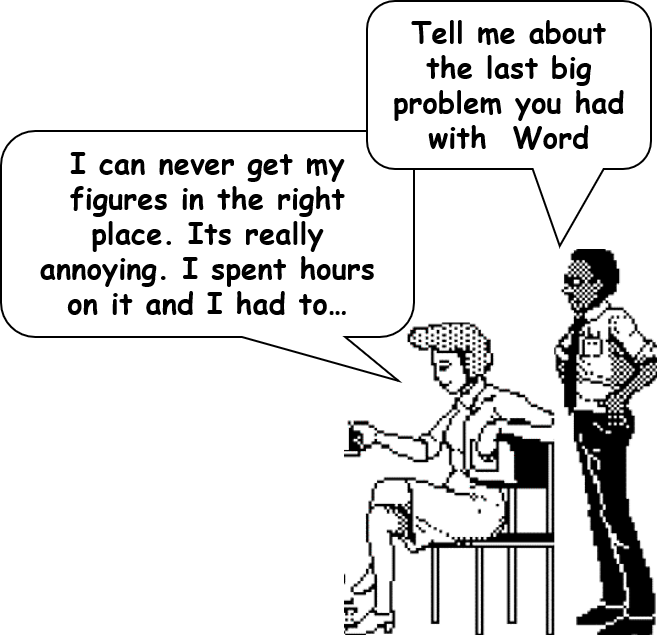
\includegraphics[scale = 0.4, right]{24_Imagine.png}
    \end{figure}
\end{frame}



% Toader Marina Adina
% slide 25
{\setbeamercolor{background canvas}{bg=background}
\setbeamercolor{normal text}{fg=Blue}
\usebeamercolor[fg]{normal text}
\begin{frame}
	\vspace{8mm}
	\textcolor{Blue}{\textbf{\large{Questionnaires and surveys}}}
    \textcolor{red}{\rule{10cm}{1mm}}

    Questionnaires / Surveys
    \begin{itemize}
      \item[\textcolor{black}{--}] preparation “expensive,” but administration cheap
      \begin{itemize}
      	\item[\textcolor{black}{•}] can reach a wide subject group (e.g. mail)
      \end{itemize}
      \item[\textcolor{black}{--}] does not require presence of evaluator
      \item[\textcolor{black}{--}] results can be quantified
    \end{itemize}
    \vspace{3mm}
     But
     \begin{itemize}
      \item[\textcolor{black}{--}] only as good as the questions asked
      \end{itemize}
    \begin{figure}[b]
    	
\includegraphics[scale = 0.4, right]{25_Imagine.png}
    \end{figure}
\end{frame}



% Toader Marina Adina
% slide 26
{\setbeamercolor{background canvas}{bg=background}
\setbeamercolor{normal text}{fg=Blue}
\usebeamercolor[fg]{normal text}
\begin{frame}	
	\vspace{8mm}
	\textcolor{Blue}{\textbf{\large{Questionnaires and surveys}}}
    \textcolor{red}{\rule{10cm}{1mm}}
    
    How
    \begin{itemize}
      \item[\textcolor{black}{--}] establish the purpose of the questionnaire
      \begin{itemize}
      	\item[\textcolor{black}{•}] what information is sought?
        \item[\textcolor{black}{•}] how would you analyze the results?
        \item[\textcolor{black}{•}] what would you do with your analysis?
      \end{itemize}
      \vspace{3mm}
      \item[\textcolor{black}{--}] do not ask questions whose answers you will not use!
      \vspace{3mm}
      \item[\textcolor{black}{--}] determine the audience you want to reach
      \vspace{3mm}
      \item[\textcolor{black}{--}] determine how would you will  deliver / collect the questionnaire
       \begin{itemize}
      	\item[\textcolor{black}{•}] on-line for computer users
        \item[\textcolor{black}{•}] web site with forms
        \item[\textcolor{black}{•}] surface mail
        \begin{itemize}
      \item[\textcolor{black}{--}] pre-addressed reply envelope gives far better response
      \end{itemize}
      \end{itemize}
      \vspace{5mm}
    \end{itemize}    
\end{frame}



% Toader Marina Adina
% slide 27
{\setbeamercolor{background canvas}{bg=background}
\setbeamercolor{normal text}{fg=Blue}
\usebeamercolor[fg]{normal text}
\begin{frame}
	\vspace{8mm}
	\textcolor{Blue}{\textbf{\large{Styles of questions}}}
    \textcolor{red}{\rule{10cm}{1mm}}
    
    Open-ended questions
    \begin{itemize}
      \item[\textcolor{black}{--}] asks for unprompted opinions
      \item[\textcolor{black}{--}] good for general subjective information
       \begin{itemize}
      	\item[\textcolor{black}{•}] but difficult to analyze rigorously
        \end{itemize} 
        \vspace{10mm}
        Can you suggest any improvements to the interfaces?
        \vspace{40mm}
    \end{itemize}    
\end{frame}



% Toader Marina Adina
% slide 28
{\setbeamercolor{background canvas}{bg=background}
\setbeamercolor{normal text}{fg=Blue}
\usebeamercolor[fg]{normal text}
\begin{frame}
	\vspace{8mm}
	\textcolor{Blue}{\textbf{\large{Styles of questions}}}
    \textcolor{red}{\rule{10cm}{1mm}}
    
    Closed questions
    \begin{itemize}
      \item[\textcolor{black}{--}] restrict respondent’s responses by supplying alternative answers
      \item[\textcolor{black}{--}] makes questionnaires a chore for respondent to fill in
      \item[\textcolor{black}{--}] can be easily analyzed
      \item[\textcolor{black}{--}] watch out for hard to interpret responses!
       \begin{itemize}
      	\item[\textcolor{black}{•}] alternative answers should be very specific
        \end{itemize} 
        \vspace{3mm}
    Do you use computers at work:\\
    {\large\hspace{5mm} \textcircled{
\includegraphics[scale = 0.6]{28_30_Imagine.png}}\hspace{2mm}often\hspace{6mm} \textcircled{}\hspace{2mm}sometimes\hspace{6mm}\textcircled{}\hspace{2mm}rarely}\\
    \textit{vs}\\
    In your typical work day,  do you use computers:\\
   {\large\hspace{5mm}\textcircled{}\hspace{2mm}over 4 hrs a day}\\ {\large\hspace{5mm}\textcircled{}\hspace{2mm}between 2 and 4 hrs daily}\\   {\large\hspace{5mm}\textcircled{
\includegraphics[scale = 0.6]{28_30_Imagine.png}}\hspace{2mm}between 1 and 2 hrs daily}\\   {\large\hspace{5mm}\textcircled{}\hspace{2mm}less than 1 hr a day}
    \end{itemize}    
\end{frame}



% Toader Marina Adina
% slide 29
{\setbeamercolor{background canvas}{bg=background}
\setbeamercolor{normal text}{fg=Blue}
\usebeamercolor[fg]{normal text}
\begin{frame}
	\vspace{8mm}
	\textcolor{Blue}{\textbf{\large{Styles of questions}}}
    \textcolor{red}{\rule{10cm}{1mm}}
    
    Scalar
    \begin{itemize}
      \item[\textcolor{black}{--}] ask user to judge a specific statement on a numeric scale
      \item[\textcolor{black}{--}] scale usually corresponds with agreement or disagreement with a statement
      \vspace{10mm}\\
      \hspace{5mm}Characters on the computer screen are:
      \begin{itemize}     \item[\textcolor{black}{--}] hard to read \hspace{15mm} easy to read
      \item[\textcolor{black}{--}] {\hspace{10mm} 1\hspace{3mm} \textcircled{2}\hspace{3mm} 3\hspace{3mm} 4\hspace{3mm} 5}
      \end{itemize}
      \vspace{25mm}
    \end{itemize}    
\end{frame}



% Toader Marina Adina
% slide 30
{\setbeamercolor{background canvas}{bg=background}
\setbeamercolor{normal text}{fg=Blue}
\usebeamercolor[fg]{normal text}
\begin{frame}
	\vspace{8mm}
	\textcolor{Blue}{\textbf{\large{Styles of questions}}}
    \textcolor{red}{\rule{10cm}{1mm}}
    
    Multi-choice
    \begin{itemize}
      \item[\textcolor{black}{--}] respondent offered a choice of explicit responses\\
      \vspace{5mm}
      How do you most often get help with the system? (tick one)
{\large\hspace{5mm}\textcircled{
\includegraphics[scale = 0.6]{28_30_Imagine.png}}\hspace{4mm}on-line manual}\\ {\large\textcircled{}\hspace{4mm}paper manual}\\      {\large\textcircled{}\hspace{4mm}ask a colleague}\\
  \vspace{5mm}
      Which types of software have you used? (tick all that apply)
{\large\hspace{5mm}\textcircled{
\includegraphics[scale = 0.6]{28_30_Imagine.png}}\hspace{4mm}word processor}\\ {\large\textcircled{}\hspace{4mm}data base}\\      {\large\textcircled{
\includegraphics[scale = 0.6]{28_30_Imagine.png}}\hspace{4mm}spreadsheet}\\
 {\large\textcircled{}\hspace{4mm}compiler}
    \end{itemize}   
\end{frame}




% Turcanu Stefan
% slide 31
{\setbeamercolor{background canvas}{bg=background}
\setbeamercolor{normal text}{fg=Blue}
\usebeamercolor[fg]{normal text}
\begin{frame}
	\vspace{8mm}
	\textcolor{Blue}{\textbf{\large{Styles of questions}}}
    \textcolor{red}{\rule{10cm}{1mm}}
    
    {\LARGE Ranked}
    \begin{itemize}
      \item[\textcolor{Blue}{--}] respondent places an ordering on items in a list 
      \item[\textcolor{Blue}{--}] useful to indicate a user’s preferences
      \item[\textcolor{Blue}{--}] forced choice
    \end{itemize}
    \vspace{5mm}
    Rank the usefulness of these methods of issuing a command\par
	(1 most useful, 2 next most useful..., 0 if not used
    \begin{itemize}
      \item[\textcolor{Blue}{\_1\_}] command line
      \item[\textcolor{Blue}{\_2\_}] menu selection
      \item[\textcolor{Blue}{\_3\_}] control key accelerator
    \end{itemize}
\end{frame}



% Turcanu Stefan
% slide 32
{\setbeamercolor{background canvas}{bg=background}
\setbeamercolor{normal text}{fg=Blue}
\usebeamercolor[fg]{normal text}
\begin{frame}
	\vspace{8mm}
	\textcolor{Blue}{\textbf{\large{Styles of questions}}}
    \textcolor{red}{\rule{10cm}{1mm}}
    
    {\LARGE Combining open-ended and closed questions}\par
    \begin{itemize}
      \item[\textcolor{Blue}{--}] gets specific response, but allows room for user’s opinion
	\end{itemize}
    \vspace{4mm}
    It is easy to recover from mistakes:\par
    \vspace{4mm}
    disagree \hspace{16mm} agree \hspace{4mm} comment:\underline{ the undo facility is} \par
    \underline{really helpful} \par
    {\large\hspace{10mm} 1\hspace{3mm} \textcircled{2}\hspace{3mm} 3\hspace{3mm} 4\hspace{3mm} 5}

\end{frame}



% Turcanu Stefan
% slide 33
{\setbeamercolor{background canvas}{bg=background}
\setbeamercolor{normal text}{fg=Blue}
\usebeamercolor[fg]{normal text}
\begin{frame}
	\vspace{8mm}
	\textcolor{Blue}{\textbf{\large{Continuous evaluation}}}
    \textcolor{red}{\rule{10cm}{1mm}}
    
    {\LARGE Monitor systems in actual use}
    \begin{itemize}
      \item[\textcolor{Blue}{--}] usually late stages of development 
        \begin{itemize}
          \item[\textcolor{Blue}{•}] ie beta releases, delivered system
        \end{itemize}
      \item[\textcolor{Blue}{--}] fix problems in next release
    \end{itemize}
    \vspace{8mm}
\begin{tikzpicture}[remember picture,overlay,shift={(current page.south east)}]
	\node[anchor=south east,xshift=0cm,yshift=2mm]{
\includegraphics[width=2cm, height=38mm]{33_Imagine.png}};
\end{tikzpicture}
    {\LARGE User feedback via gripe lines}
    \begin{itemize}
      \item[\textcolor{Blue}{--}] users can provide feedback to designers while using the system
      \begin{itemize}
        \item[\textcolor{Blue}{•}] help desks
        \item[\textcolor{Blue}{•}] bulletin boards
        \item[\textcolor{Blue}{•}] email
        \item[\textcolor{Blue}{•}] built-in gripe facility
      \end{itemize}
    \end{itemize}
	\vspace{3mm}
	\begin{itemize}
      \item[\textcolor{Blue}{--}] best combined with trouble-shooting facility
        \begin{itemize}
          \item[\textcolor{Blue}{•}] users always get a response (solution?) to their gripes
        \end{itemize}
    \end{itemize}
\end{frame}



% Turcanu Stefan
% slide 34
{\setbeamercolor{background canvas}{bg=background}
\setbeamercolor{normal text}{fg=Blue}
\usebeamercolor[fg]{normal text}
\begin{frame}
	\vspace{8mm}
	\textcolor{Blue}{\textbf{\large{Continuous evaluation}}}
    \textcolor{red}{\rule{10cm}{1mm}}
    
    {\Large Case/field studies}
    \begin{itemize}
      \item[\textcolor{Blue}{--}] careful study of "system usage" at the site
      \item[\textcolor{Blue}{--}] good for seeing "real life" use
      \item[\textcolor{Blue}{--}] external observer monitors behavior 
      \item[\textcolor{Blue}{--}] site visits
    \end{itemize}
    \vspace{12mm}
    \begin{figure}[b]
    	
\includegraphics[scale = 0.5, right]{34_Imagine.png}
    \end{figure}
\end{frame}


% Turcanu Stefan
% slide 35
{\setbeamercolor{background canvas}{bg=background}
\setbeamercolor{normal text}{fg=Blue}
\usebeamercolor[fg]{normal text}
\begin{frame}
	\vspace{8mm}
	\textcolor{Blue}{\textbf{\large{Ethics}}}
    \textcolor{red}{\rule{10cm}{1mm}}
    
    \begin{figure}[b]
    	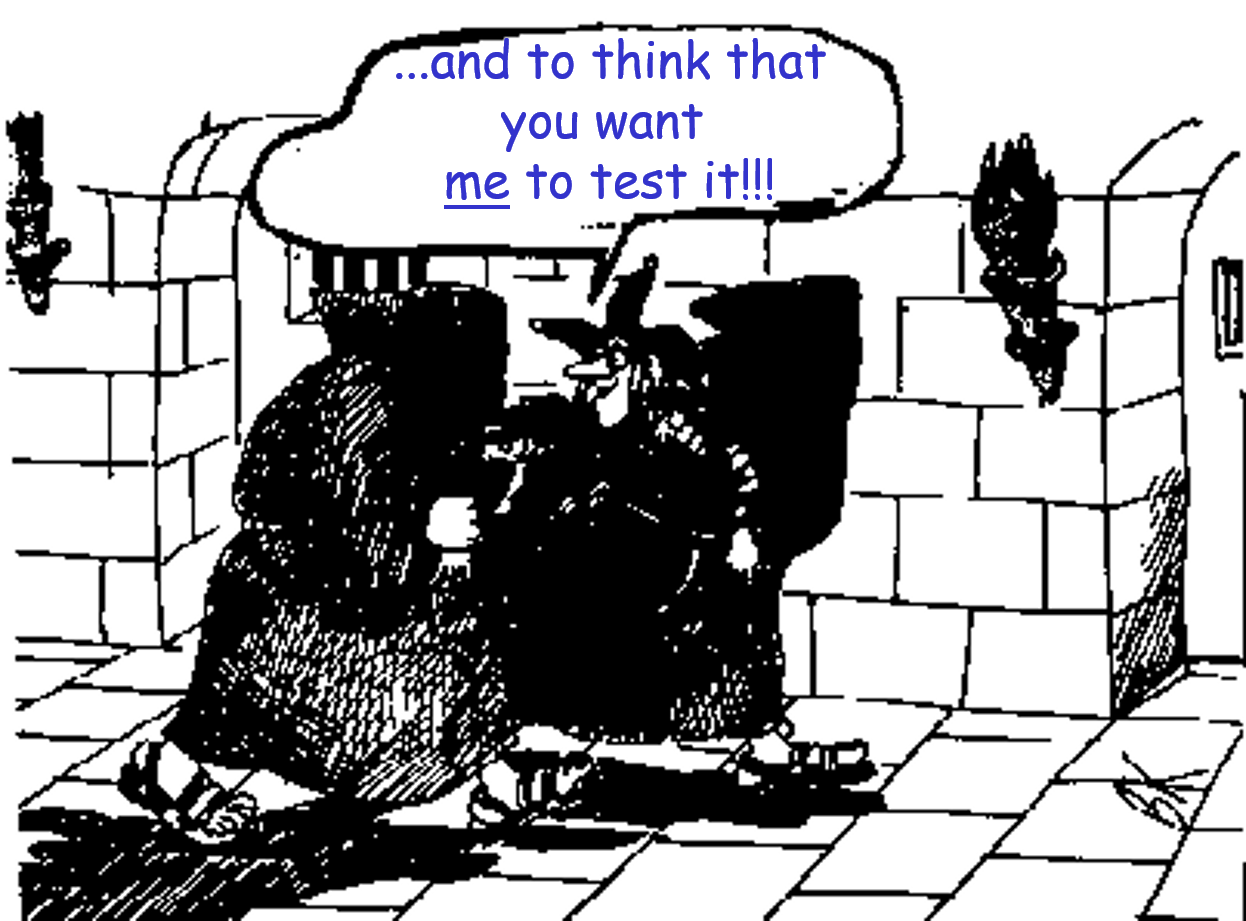
\includegraphics[scale = 0.45, center]{35_Imagine.png}
    \end{figure}
\end{frame}



% Turcanu Stefan
% slide 36
{\setbeamercolor{background canvas}{bg=background}
\setbeamercolor{normal text}{fg=Blue}
\usebeamercolor[fg]{normal text}
\begin{frame}
	\vspace{8mm}
	\textcolor{Blue}{\textbf{\large{Ethics}}}
    \textcolor{red}{\rule{10cm}{1mm}}

  \begin{tikzpicture}[remember picture,overlay,shift={(current page.north east)}]
      \node[anchor=north east,xshift=0cm,yshift=0cm]{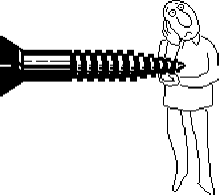
\includegraphics[width=4cm, height=24mm]{36_Imagine.png}};
  \end{tikzpicture}

  {\Large Testing can be a distressing experience}
  \begin{itemize}
    \item[\textcolor{Blue}{--}] pressure to perform, errors inevitable
    \item[\textcolor{Blue}{--}] feelings of inadequacy
    \item[\textcolor{Blue}{--}] competition with other subjects
  \end{itemize}
  \vspace{12mm}
  {\Large Golden rule}
  \begin{itemize}
    \item[\textcolor{Blue}{--}] subjects should always be treated with respect
  \end{itemize}
\end{frame}



% Turcanu Stefan
% slide 37
{\setbeamercolor{background canvas}{bg=background}
\setbeamercolor{normal text}{fg=Blue}
\usebeamercolor[fg]{normal text}
\begin{frame}
	\vspace{8mm}
	\textcolor{Blue}{\textbf{\large{Ethics - before the test}}}
    \textcolor{red}{\rule{10cm}{1mm}}
    
    {\Large Don’t waste the user’s time}
	\begin{itemize}
    	\item[\textcolor{Blue}{--}]use pilot tests to debug experiments, questionnaires etc
    	\item[\textcolor{Blue}{--}]have everything ready before the user shows up
	\end{itemize}
    {\Large Make users feel comfortable}
    \begin{itemize}
    	\item[\textcolor{Blue}{--}]emphasize that it is the system that is being tested, not the user
    	\item[\textcolor{Blue}{--}]acknowledge that the software may have problems
    	\item[\textcolor{Blue}{--}]let users know they can stop at any time
	\end{itemize}
    {\Large Maintain privacy}
    \begin{itemize}
    	\item[\textcolor{Blue}{--}]tell user that individual test results will be completely confidential
	\end{itemize}
    {\Large Inform the user}
    \begin{itemize}
    	\item[\textcolor{Blue}{--}]explain any monitoring that is being used
    	\item[\textcolor{Blue}{--}]answer all user’s questions (but avoid bias)
	\end{itemize}
    {\Large Only use volunteers}
    \begin{itemize}
    	\item[\textcolor{Blue}{--}]user must sign an informed consent form
    \end{itemize}
\end{frame}



% Turcanu Stefan
% slide 38
{\setbeamercolor{background canvas}{bg=background}
\setbeamercolor{normal text}{fg=Blue}
\usebeamercolor[fg]{normal text}
\begin{frame}
	\vspace{8mm}
	\textcolor{Blue}{\textbf{\large{Ethics - during the test}}}
    \textcolor{red}{\rule{10cm}{1mm}}
    
	{\Large Don't waste the user's time}\par
    \begin{itemize}
		\item[\textcolor{Blue}{--}]never have the user perform unnecessary tasks
	\end{itemize}
	{\Large Make users comfortable}\par
	\begin{itemize}
		\item[\textcolor{Blue}{--}]try to give user an early success experience
		\item[\textcolor{Blue}{--}]keep a relaxed atmosphere in the room 
		\item[\textcolor{Blue}{--}]coffee, breaks, etc
		\item[\textcolor{Blue}{--}]hand out test tasks one at a time
		\item[\textcolor{Blue}{--}]never indicate displeasure with the user’s performance
		\item[\textcolor{Blue}{--}]avoid disruptions
		\item[\textcolor{Blue}{--}]stop the test if it becomes too unpleasant
        \newline
    \end{itemize}	

	{\Large Maintain privacy}\par
    \begin{itemize}
		\item[\textcolor{Blue}{--}]do not allow the user’s management to observe the test
    \end{itemize}
\end{frame}



% Vedinas Roxana
% slide 39
{\setbeamercolor{background canvas}{bg=background}
\setbeamercolor{normal text}{fg=Blue}
\usebeamercolor[fg]{normal text}
\begin{frame}
	\vspace{8mm}
	\textcolor{Blue}{\textbf{\large{Ethics - after the test}}}
    \textcolor{red}{\rule{10cm}{1mm}}
    
	{\Large Make the users feel comfortable}\par
    \begin{itemize}
		\item[\textcolor{Blue}{--}] state that the user has helped you find areas of improvement
    \end{itemize}
   \bigskip
	{\Large Inform the user}\par
    \begin{itemize}
		\item[\textcolor{Blue}{--}] answer particular questions about the experiment that could have biased the results before
    \end{itemize}	
    \bigskip
	{\Large Maintain privacy}\par
    \begin{itemize}
		\item[\textcolor{Blue}{--}] never report results in a way that individual users can be identified
		\item[\textcolor{Blue}{--}] only show videotapes outside the research group with the user’s permission
    \end{itemize}
\end{frame}



% Vedinas Roxana
% slide 40
{\setbeamercolor{background canvas}{bg=background}
\setbeamercolor{normal text}{fg=Blue}
\usebeamercolor[fg]{normal text}
\begin{frame}
	\vspace{8mm}
	\textcolor{Blue}{\textbf{\large{What you now know}}}
    \textcolor{red}{\rule{10cm}{1mm}}
    
	{\Large Debug designs by observing how people use them}\par
    \begin{itemize}
		\item[\textcolor{Blue}{--}] quickly exposes successes and problems
        \item[\textcolor{Blue}{--}] specific methods reveal what a person is thinking
        \item[\textcolor{Blue}{--}] but naturalistic vs laboratory evaluations is a tradeoff
    \end{itemize}
   \bigskip
	{\Large Methods include}\par
    \begin{itemize}
		\item[\textcolor{Blue}{--}] conceptual model extraction
        \item[\textcolor{Blue}{--}] direct observation
        \begin{itemize}
        \item[\textcolor{Blue}{•}] think-aloud
        \item[\textcolor{Blue}{•}] constructive interaction/co-discovery
      \end{itemize}
        \item[\textcolor{Blue}{--}] query via interviews, retrospective testing and questionnaires
        \item[\textcolor{Blue}{--}] continuous evaluation via user feedback and field studies
    \end{itemize}	
    \bigskip
	{\Large Ethics are important}\par
\end{frame}



% Vedinas Roxana
% slide 41
{\setbeamercolor{background canvas}{bg=background}
\setbeamercolor{normal text}{fg=Blue}
\usebeamercolor[fg]{normal text}
\begin{frame} 
	\vspace{8mm}
	\textcolor{Blue}{\textbf{\large{Interface Design and Usability Engineering}}}
    \textcolor{red}{\rule{10cm}{1mm}}
    
\begin{figure}[h] \begin{flushright}
	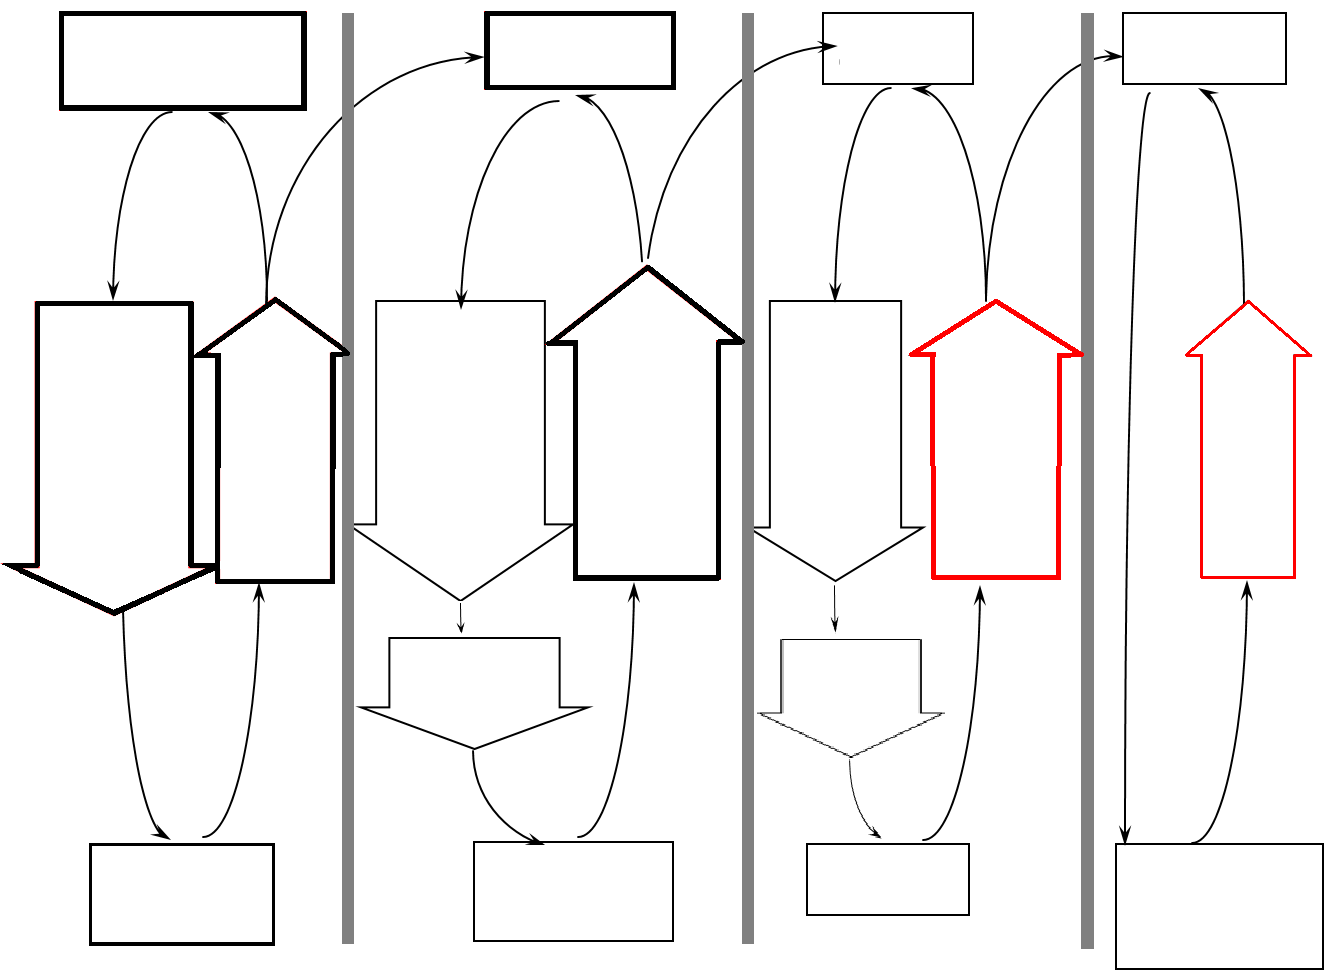
\includegraphics[width=0.98\textwidth]{41_picture.png}
\end{flushright}
\end{figure}
\leavevmode\makebox(0,0){\put(-27,450){\selectfont{\textbf{\footnotesize Goals:}}}}
\leavevmode\makebox(0,0){\put(-30,280){\selectfont{\textbf{\footnotesize Methods:}}}}
\leavevmode\makebox(0,0){\put(-33,80){\selectfont{\textbf{\footnotesize Products:}}}}
%prima coloana
\leavevmode\makebox(0,0){\put(10,470){\selectfont{\textbf{\tiny Articulate:}}}}
\leavevmode\makebox(0,0){\put(9,460){\selectfont{\textbf{\tiny *who users are}}}}
\leavevmode\makebox(0,0){\put(5,450){\selectfont{\textbf{\tiny *their key tasks }}}}
\leavevmode\makebox(0,0){\put(-3,332){\selectfont{\tiny Task }}}
\leavevmode\makebox(0,0){\put(-7,320){\selectfont{\tiny centered }}}
\leavevmode\makebox(0,0){\put(-10,307){\selectfont{\tiny system }}}
\leavevmode\makebox(0,0){\put(-14,295){\selectfont{\tiny design }}}
\leavevmode\makebox(0,0){\put(-23,275){\selectfont{\tiny Participatory }}}
\leavevmode\makebox(0,0){\put(-20,265){\selectfont{\tiny design }}}
\leavevmode\makebox(0,0){\put(-25,250){\selectfont{\tiny User- }}}
\leavevmode\makebox(0,0){\put(-28,240){\selectfont{\tiny centered }}}
\leavevmode\makebox(0,0){\put(-32,230){\selectfont{\tiny design }}}
\leavevmode\makebox(0,0){\put(-27,80){\selectfont{\textbf{\tiny User and task }}}}
\leavevmode\makebox(0,0){\put(-26,70){\selectfont{\textbf{\tiny description }}}}
\leavevmode\makebox(0,0){\put(-5,280){\selectfont{\tiny Evaluate }}}
\leavevmode\makebox(0,0){\put(-8,265){\selectfont{\tiny tasks }}}
%a doua coloana
\leavevmode\makebox(0,0){\put(50,470){\selectfont{\textbf{\tiny Brainstorm }}}}
\leavevmode\makebox(0,0){\put(48,460){\selectfont{\textbf{\tiny design }}}}
\leavevmode\makebox(0,0){\put(15,330){\selectfont{\textcolor{gray}{\tiny Psychology }}}}
\leavevmode\makebox(0,0){\put(12,320){\selectfont{\textcolor{gray}{\tiny of everyday }}}}
\leavevmode\makebox(0,0){\put(8,310){\selectfont{\textcolor{gray}{\tiny things }}}}
\leavevmode\makebox(0,0){\put(5,290){\selectfont{\tiny User }}}
\leavevmode\makebox(0,0){\put(2,280){\selectfont{\tiny involvement }}}
\leavevmode\makebox(0,0){\put(-3,260){\selectfont{\textcolor{gray}{\tiny Representation }}}}
\leavevmode\makebox(0,0){\put(-4,250){\selectfont{\textcolor{gray}{\tiny metaphors }}}}
\leavevmode\makebox(0,0){\put(-5,180){\selectfont{\tiny low fidelity }}}
\leavevmode\makebox(0,0){\put(-8,170){\selectfont{\tiny prototyping }}}
\leavevmode\makebox(0,0){\put(-11,160){\selectfont{\tiny methods }}}
\leavevmode\makebox(0,0){\put(5,90){\selectfont{\textbf{\tiny Throw-away }}}}
\leavevmode\makebox(0,0){\put(2,80){\selectfont{\textbf{\tiny paper }}}}
\leavevmode\makebox(0,0){\put(-1,70){\selectfont{\textbf{\tiny prototypes }}}}
\leavevmode\makebox(0,0){\put(13,320){\selectfont{\tiny Participatory }}}
\leavevmode\makebox(0,0){\put(10,310){\selectfont{\tiny interaction }}}
\leavevmode\makebox(0,0){\put(7,280){\selectfont{\tiny Task }}}
\leavevmode\makebox(0,0){\put(5,270){\selectfont{\tiny scenario }}}
\leavevmode\makebox(0,0){\put(1,260){\selectfont{\tiny walk- }}}
\leavevmode\makebox(0,0){\put(-2,250){\selectfont{\tiny through }}}
%a treia coloana
\leavevmode\makebox(0,0){\put(52,470){\selectfont{\textbf{\tiny Redefined }}}}
\leavevmode\makebox(0,0){\put(49,460){\selectfont{\textbf{\tiny designs }}}}
\leavevmode\makebox(0,0){\put(30,340){\selectfont{\textcolor{gray}{\tiny Graphical }}}}
\leavevmode\makebox(0,0){\put(30,330){\selectfont{\textcolor{gray}{\tiny screen }}}}
\leavevmode\makebox(0,0){\put(25,320){\selectfont{\textcolor{gray}{\tiny design }}}}
\leavevmode\makebox(0,0){\put(20,300){\selectfont{\textcolor{gray}{\tiny Interface }}}}
\leavevmode\makebox(0,0){\put(15,290){\selectfont{\textcolor{gray}{\tiny guidelines }}}}
\leavevmode\makebox(0,0){\put(13,270){\selectfont{\textcolor{gray}{\tiny Style }}}}
\leavevmode\makebox(0,0){\put(10,260){\selectfont{\textcolor{gray}{\tiny guides }}}}
\leavevmode\makebox(0,0){\put(5,180){\selectfont{\tiny high fidelity }}}
\leavevmode\makebox(0,0){\put(2,170){\selectfont{\tiny prototyping }}}
\leavevmode\makebox(0,0){\put(-1,160){\selectfont{\tiny methods }}}
\leavevmode\makebox(0,0){\put(5,90){\selectfont{\textbf{\tiny Testable }}}}
\leavevmode\makebox(0,0){\put(2,80){\selectfont{\textbf{\tiny prototypes }}}}
\leavevmode\makebox(0,0){\put(23,320){\selectfont{\textbf{\textcolor{red}{\tiny Usability }}}}}
\leavevmode\makebox(0,0){\put(20,310){\selectfont{\textbf{\textcolor{red}{\tiny testing }}}}}
\leavevmode\makebox(0,0){\put(15,280){\selectfont{\textcolor{gray}{\tiny Heuristic }}}}
\leavevmode\makebox(0,0){\put(12,270){\selectfont{\textcolor{gray}{\tiny evaluation }}}}
%a patra coloana
\leavevmode\makebox(0,0){\put(55,470){\selectfont{\textbf{\textcolor{gray}{\tiny Completed }}}}}
\leavevmode\makebox(0,0){\put(52,460){\selectfont{\textbf{\textcolor{gray}{\tiny designs }}}}}
\leavevmode\makebox(0,0){\put(65,310){\selectfont{\textcolor{red}{\tiny Field }}}}
\leavevmode\makebox(0,0){\put(60,300){\selectfont{\textcolor{red}{\tiny testing }}}}
\leavevmode\makebox(0,0){\put(40,90){\selectfont{\textbf{\textcolor{gray}{\tiny Alpha/beta }}}}}
\leavevmode\makebox(0,0){\put(36,80){\selectfont{\textbf{\textcolor{gray}{\tiny systems or }}}}}
\leavevmode\makebox(0,0){\put(33,70){\selectfont{\textbf{\textcolor{gray}{\tiny complete }}}}}
\leavevmode\makebox(0,0){\put(29,60){\selectfont{\textbf{\textcolor{gray}{\tiny specification }}}}}
\end{frame}
}



{\setbeamercolor{background canvas}{bg=background}
\setbeamercolor{normal text}{fg=Blue}
\usebeamercolor[fg]{normal text}
\begin{frame}
	\vspace{8mm}
	\textcolor{Blue}{\textbf{\Large{*Bibliography}}}
    \textcolor{red}{\rule{10cm}{1mm}}

        \begin{itemize}
        	\item[{$\bullet$}] Saul Greenberg, \textbf{Designing with the user. User centered design and Prototyping}, University of Calgary, Canada

        	\url{http://pages.cpsc.ucalgary.ca/~saul/481/}
        	\newline
        	 
        	\item[{$\bullet$}] Keith Andrews, \textbf{Human Computer Interaction, Chapter 3. Usability Engineering, Chapter 9. Usability Testing Methods}, TU Graz, Austria

        	\url{https://courses.isds.tugraz.at/hci/hci.pdf}                			\newline
     	\end{itemize}
\end{frame}



\end{document}